% In this section, the layer is described in some detail in terms of its specific subsystems. Describe each of the layers and its subsystems in a separate chapter/major subsection of this document. The content of each subsystem description should be similar. Include in this section any special considerations and/or trade-offs considered for the approach you have chosen.

The pathfinding subsystem manages the components or modules within a larger pathfinding system that handles specific aspects of the 

\subsection{Static Map Subsystem}
The Static Map subsystem allows the display of the LiDAR range as a grid of cells and allows them to be marked as either traversable or non-traversable, as needed.

% This section should be a general description of a particular subsystem for the given layer. For most subsystems, an extract of the architectural block diagram with data flows is useful. This should consist of the subsystem being described and those subsystems with which it communicates.


%%%%%%%%%%%%%%%%%%%%%%%%%%%%%%%%%%%%%%%%%%%%%%%%%%%%%%%%%%%%%%%%%%%%%%%%%%%%
%   Change the graphic here. Put your image in the 'images' folder
%   and update the name from 'images/test_image' to your image name
\begin{figure}[h!]
	\centering
 	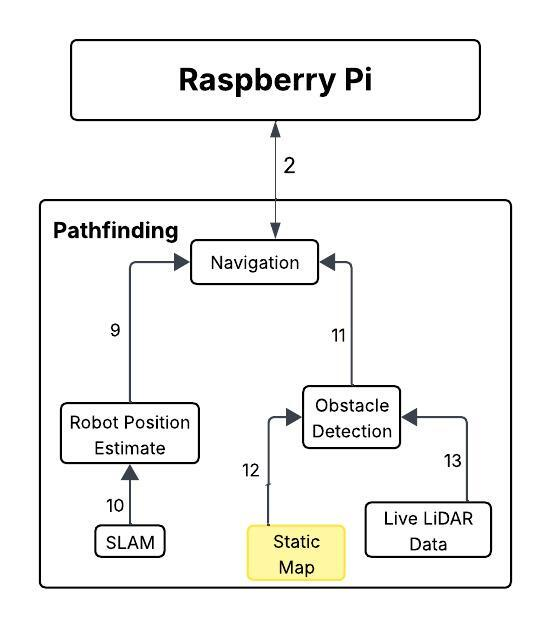
\includegraphics[width=0.80\textwidth]{images/pathfinding 2/Data_Flow_StaticMap.jpeg}
 \caption{Pathfinding Subsystem - Static Map} % Be sure to change the caption.
\end{figure}

\subsubsection{Assumptions}
% Any assumptions made in the definition of the subsystem should be listed and described. Pay particular attention to assumptions concerning interfaces and interactions with other layers.

Static Map assumes that the Obstacle Detection will be functional, and there will not be dynamic obstacles or other movement during pathfinding.
\subsubsection{Responsibilities}
% Each of the responsibilities/features/functions/services of the subsystem as identified in the architectural summary must be expanded to more detailed responsibilities. These responsibilities form the basis for the identification of the finer-grained responsibilities of the layer's internal subsystems. Clearly describe what each subsystem does.

The static map creates a map using the SlamTec LiDAR to than feed into the Obstacle Detection Subystem, so that it can create a costmap.
\subsubsection{Subsystem Interfaces}
% Each of the inputs and outputs for the subsystem are defined here. Create a table with an entry for each labelled interface that connects to this subsystem. For each entry, describe any incoming and outgoing data elements will pass through this interface.

\begin {table}[H]
\caption {Pathfinding Subsystem - Static Map} 
\begin{center}
    \begin{tabular}{ | p{1.2cm} | p{6cm} | p{3cm} | p{3cm} |}
    \hline
    ID & Description & Inputs & Outputs \\ \hline
    \#12 & Data converts Laser Scan into Map & \pbox{3cm}{N/A} & \pbox{3cm}{Map (.yaml file) }  \\ \hline

    \end{tabular}
\end{center}
\end{table}

\newpage

\subsection{Obstacle Detection Subsystems}
The obstacle detection subsystem is designed to process feedback from the LiDAR, identifying objects within its range and marking them as impassable when necessary.
%%%%%%%%%%%%%%%%%%%%%%%%%%%%%%%%%%%%%%%%%%%%%%%%%%%%%%%%%%%%%%%%%%%%%%%%%%%%
%   Change the graphic here. Put your image in the 'images' folder
%   and update the name from 'images/test_image' to your image name
\begin{figure}[h!]
	\centering
 	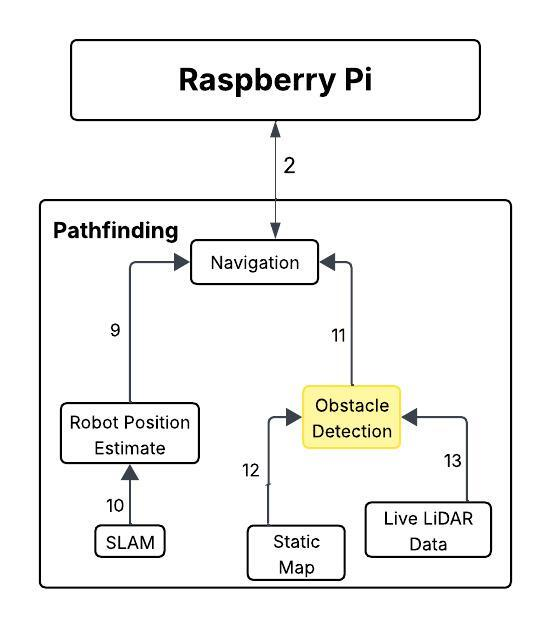
\includegraphics[width=0.60\textwidth]{images/pathfinding 2/Data_Flow_ObstacleD.jpeg}
 \caption{Pathfinding Subsystem - Obstacle Detection} % Be sure to change the caption.
\end{figure}

\subsubsection{Assumptions}
% Any assumptions made in the definition of the subsystem should be listed and described. Pay particular attention to assumptions concerning interfaces and interactions with other layers.
The rover will be able to register static and dynamic obstacles and be detected with LiDAR.
\subsubsection{Responsibilities}
% Each of the responsibilities/features/functions/services of the subsystem as identified in the architectural summary must be expanded to more detailed responsibilities. These responsibilities form the basis for the identification of the finer-grained responsibilities of the layer's internal subsystems. Clearly describe what each subsystem does.

The rover will be able to detect obstacles and update the graph representation Subsystem by marking a cell as untraversable. The obstacle detection subsystem should also be able to be integrated with LiDAR and other sensors. If the close-range sensors get triggered the rover should halt movement and retreat a set distance before reactivating its pathfinding.

The pathfinding algorithm creates a grid using the map the static map subsystem provided, representing the environment with the LiDAR Range. The grid will contain nodes that contain properties such as: 
\begin{itemize}
  \item Traverability (true/false).
  \item Coordinates in world space.
\end{itemize}
\subsubsection{Subsystem Interfaces}
% Each of the inputs and outputs for the subsystem are defined here. Create a table with an entry for each labelled interface that connects to this subsystem. For each entry, describe any incoming and outgoing data elements will pass through this interface.


\begin{table}[H]
\caption{Pathfinding Subsystem - Obstacle Detection} 
\begin{center}
    \begin{tabular}{ | p{1.8cm} | p{8cm} | p{2cm} | p{3cm} |}
    \hline
    ID & Description & Inputs & Outputs  \\ \hline
    \#11 & Algorithm will send a signal to the navigation. & N/A & Marked Obstacles \\ \hline
    \#12 & Algorithm combines the data from map. & Map Data  & N/A \\ \hline
    \#13 & Algorithm combines the data from LiDAR. & Scan Data & N/A \\ \hline
    \end{tabular}
\end{center}
\end{table}


\newpage

\subsection{Navigation Subsystems}
The Navigation Subsystem enables the Roam\_Bot to autonomously navigate the environment by combining real-time position data from the Robot Position Estimate Subsystem with obstacle information from the SLAM-generated map. It generates an optimal path through the terrain, considering both the robot's current pose and the locations of obstacles, and continuously adjusts the path as the environment changes.
%%%%%%%%%%%%%%%%%%%%%%%%%%%%%%%%%%%%%%%%%%%%%%%%%%%%%%%%%%%%%%%%%%%%%%%%%%%%
%   Change the graphic here. Put your image in the 'images' folder
%   and update the name from 'images/test_image' to your image name
\begin{figure}[h!]
	\centering
 	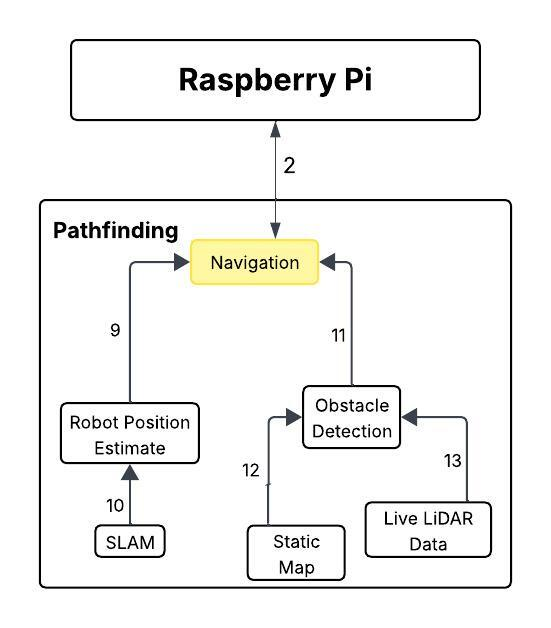
\includegraphics[width=0.60\textwidth]{images/pathfinding 2/Data_Flow_Navigation.jpeg}
 \caption{Pathfinding Subsystem - Navigation} % Be sure to change the caption.
\end{figure}

\subsubsection{Assumptions}
% Any assumptions made in the definition of the subsystem should be listed and described. Pay particular attention to assumptions concerning interfaces and interactions with other layers.

The pathfinding algorithm requires that the graph is already constructed, and LiDAR is active.
\subsubsection{Responsibilities}
% Each of the responsibilities/features/functions/services of the subsystem as identified in the architectural summary must be expanded to more detailed responsibilities. These responsibilities form the basis for the identification of the finer-grained responsibilities of the layer's internal subsystems. Clearly describe what each subsystem does.

The pathfinding algorithm calculates either the optimal or heuristic-based path from a start to end node. The pathfinding algorithms should also allow for multiple algorithms, such as A*, Dijkstra's, Breadth-First-Search, etc. While also handling static and dynamic obstacles.
\subsubsection{Subsystem Interfaces}
% Each of the inputs and outputs for the subsystem are defined here. Create a table with an entry for each labelled interface that connects to this subsystem. For each entry, describe any incoming and outgoing data elements will pass through this interface.

\begin{table}[H]
\caption{Pathfinding Subsystem - Navigation} 
\begin{center}
    \begin{tabular}{ | p{1.8cm} | p{8cm} | p{2cm} | p{3cm} |}
    \hline
    ID & Description & Inputs & Outputs  \\ \hline
    \#2 & Sending movement decision to Raspberry Pi. & N/A & Data to TM4C (Microcontroller) \\ \hline
    \#9 & Receives approximate position odometry. & Position from SLAM & N/A \\ \hline
    \#11 & Receives obstacles detected from scan. & Obstacle Detection & N/A \\ \hline
    \end{tabular}
\end{center}
\end{table}

\newpage


\subsection{Live LiDAR Data Subsystems}
The LiDAR subsystem is implemented as a ROS package that interfaces with and drives the LiDAR hardware module, providing the Roam\_Bot with real time scan data used to perceive and interpret the surrounding terrain.
%%%%%%%%%%%%%%%%%%%%%%%%%%%%%%%%%%%%%%%%%%%%%%%%%%%%%%%%%%%%%%%%%%%%%%%%%%%%
%   Change the graphic here. Put your image in the 'images' folder
%   and update the name from 'images/test_image' to your image name
\begin{figure}[h!]
	\centering
 	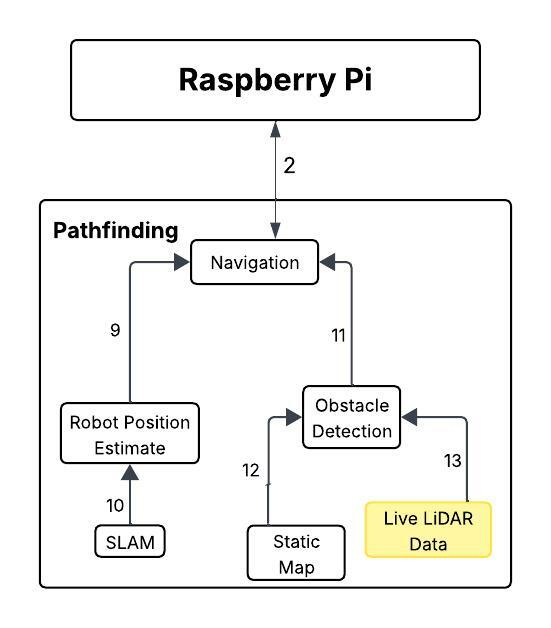
\includegraphics[width=0.60\textwidth]{images/pathfinding 2/Data_Flow_LiveLiDAR.jpeg}
 \caption{Pathfinding Subsystem - Live LiDAR Data} % Be sure to change the caption.
\end{figure}

\subsubsection{Assumptions}
% Any assumptions made in the definition of the subsystem should be listed and described. Pay particular attention to assumptions concerning interfaces and interactions with other layers.
\begin{itemize}
    \item Static Obstacles are Detected Within Range
    \item Robot Operates on a Relatively Flat Plane
    \item Costmap is Regularly Updated with LiDAR Data
    \item No Excessive Sensor Noise or Clutter
\end{itemize}

The LiDAR subsystem requires that the Roam\_Bot be turned on.
\subsubsection{Responsibilities}
% Each of the responsibilities/features/functions/services of the subsystem as identified in the architectural summary must be expanded to more detailed responsibilities. These responsibilities form the basis for the identification of the finer-grained responsibilities of the layer's internal subsystems. Clearly describe what each subsystem does.

The LiDAR subsystem takes the input given by its sensors and sends all relevant information to the Obstacle Detection subsystem, which creates a costmap.

\subsubsection{Subsystem Interfaces}


% Each of the inputs and outputs for the subsystem are defined here. Create a table with an entry for each labelled interface that connects to this subsystem. For each entry, describe any incoming and outgoing data elements will pass through this interface.

\begin {table}[H]
\caption {Pathfinding Subsystem - Live LiDAR Data} 
\begin{center}
    \begin{tabular}{ | p{1cm} | p{6cm} | p{3cm} | p{3cm} |}
    \hline
    ID & Description & Inputs & Outputs \\ \hline
    \#13 &  The LiDAR subsystem will transmit laser scan data to the Obstacle Detection subsystem, which will process the input, convert it into a structured grid, and divide it into individual cells for further analysis.
    & \pbox{3cm}{N/A} & \pbox{3cm}{Obstacle Detection}  \\ \hline
    \end{tabular}
\end{center}
\end{table}

\newpage



\subsection{Robot Position Estimate Subsystem}

The Robot Position Estimate Subsystem is responsible for determining the robot's current pose (position and orientation) within a map generated by SLAM. It continuously updates the pose using LiDAR data and provides this information to the Navigation Decision Subsystem for path planning and movement control.

\begin{figure}[h!]
	\centering
 	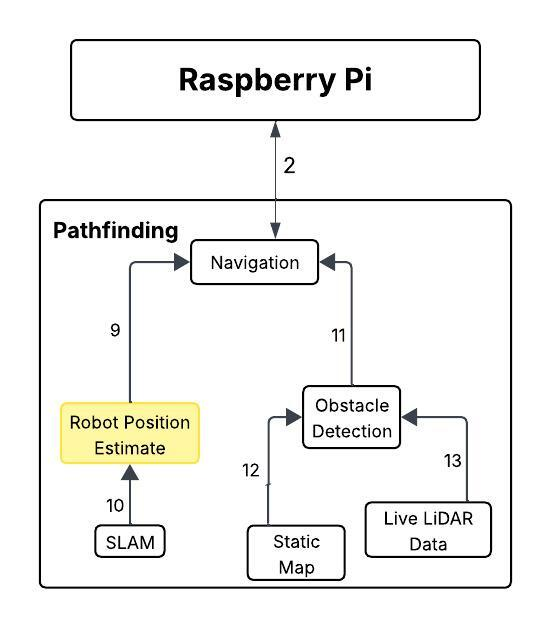
\includegraphics[width=0.80\textwidth]{images/pathfinding 2/Data_Flow_RobotPosition.jpeg}
 	\caption{Pathfinding Subsystem - Position Estimate}
\end{figure}

\subsubsection{Assumptions}

\begin{itemize}
    \item SLAM is functioning correctly and consistently receives LiDAR input.
    \item The robot operates in a primarily static environment suitable for SLAM-based localization.
    \item The initial pose is known or initialized at the origin.
    \item The Raspberry Pi is fully operational and can run SLAM in real time.
\end{itemize}

\subsubsection{Responsibilities}

The Robot Position Estimate Subsystem performs the following functions:
\begin{itemize}
  \item Accepts pose data from the SLAM subsystem.
  \item Maintains the robot’s estimated pose in the global coordinate frame.
  \item Provides updated pose data to the Navigation Decision Subsystem for route planning and motion.
  \item Supports coordinate conversion as necessary for integration with grid-based navigation.
\end{itemize}

\subsubsection{Subsystem Interfaces}

\begin{table}[H]
\caption{Pathfinding Subsystem - Position Estimate}
\begin{center}
    \begin{tabular}{ | p{1.5cm} | p{6cm} | p{3cm} | p{3cm} |}
    \hline
    ID & Description & Inputs & Outputs \\ \hline
    \#9  & Current estimated robot pose for navigation decisions & N/A & Robot Pose\\ \hline
    \#10 & Pose data provided by SLAM & SLAM Pose & N/A \\ \hline
    \end{tabular}
\end{center}
\end{table}

\newpage






\subsection{SLAM}
The SLAM subsystem processes data to simultaneously localize the robot within an environment and build a global occupancy grid map. This enables the Robot Position Estimate Subsystem to determine the robot's real time pose (x, y, θ) in relation to the mapped surroundings, which is critical for accurate navigation and planning.

% This section should be a general description of a particular subsystem for the given layer. For most subsystems, an extract of the architectural block diagram with data flows is useful. This should consist of the subsystem being described and those subsystems with which it communicates.




%%%%%%%%%%%%%%%%%%%%%%%%%%%%%%%%%%%%%%%%%%%%%%%%%%%%%%%%%%%%%%%%%%%%%%%%%%%%
%   Change the graphic here. Put your image in the 'images' folder
%   and update the name from 'images/test_image' to your image name
\begin{figure}[h!]
	\centering
 	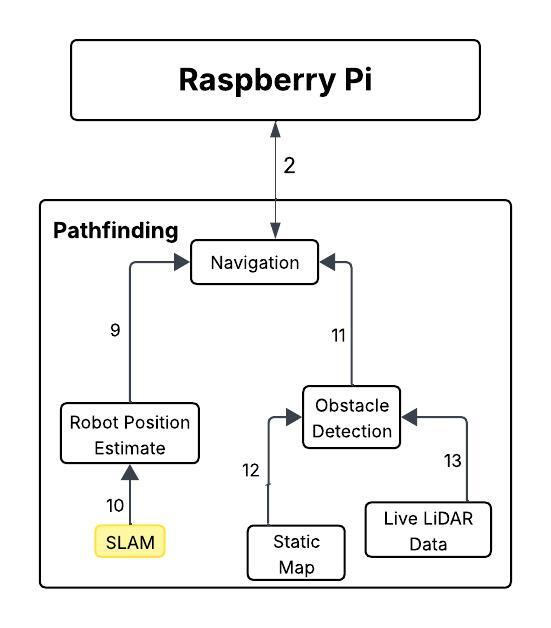
\includegraphics[width=0.80\textwidth]{images/pathfinding 2/Data_Flow_SLAM.jpeg}
 \caption{Pathfinding Subsystem - SLAM} % Be sure to change the caption.
\end{figure}

\subsubsection{Assumptions}
% Any assumptions made in the definition of the subsystem should be listed and described. Pay particular attention to assumptions concerning interfaces and interactions with other layers.
\begin{itemize}
    \item ROS2 Jazzy is installed on the Raspberry Pi 5.
    \item Nav2 Jazzy is installed on the Raspberry Pi 5.
    \item The Static Map is locatable on the Raspberry Pi 5.
    \item Robot operates on a relatively flat plane.
\end{itemize}
\subsubsection{Responsibilities}
% Each of the responsibilities/features/functions/services of the subsystem as identified in the architectural summary must be expanded to more detailed responsibilities. These responsibilities form the basis for the identification of the finer-grained responsibilities of the layer's internal subsystems. Clearly describe what each subsystem does.

The responsibilites that SLAM uses is:
\begin{itemize}
  \item Real-Time Map Building: (Mapping) Continuously generates a 2D or 3D map of the environment based on sensor data (typically LiDAR or depth camera).
  \item Robot Localization: Estimates the robot's pose (x, y, θ) in the global map frame in real time. Uses scan matching or visual feature matching to align sensor data with the evolving map.
\end{itemize}
\subsubsection{Subsystem Interfaces}
% Each of the inputs and outputs for the subsystem are defined here. Create a table with an entry for each labelled interface that connects to this subsystem. For each entry, describe any incoming and outgoing data elements will pass through this interface.

\begin {table}[H]
\caption {Pathfinding Subsystem - SLAM} 
\begin{center}
    \begin{tabular}{ | p{1.2cm} | p{6cm} | p{3cm} | p{3cm} |}
    \hline
    ID & Description & Inputs & Outputs \\ \hline
    \#10 & Slam's localization function outputs the robot's position estimate & \pbox{3cm}{N/A} & \pbox{3cm}{SLAM Pose}  \\ \hline

    \end{tabular}
\end{center}
\end{table}